\documentclass[1p]{elsarticle_modified}
%\bibliographystyle{elsarticle-num}

%\usepackage[colorlinks]{hyperref}
%\usepackage{abbrmath_seonhwa} %\Abb, \Ascr, \Acal ,\Abf, \Afrak
\usepackage{amsfonts}
\usepackage{amssymb}
\usepackage{amsmath}
\usepackage{amsthm}
\usepackage{scalefnt}
\usepackage{amsbsy}
\usepackage{kotex}
\usepackage{caption}
\usepackage{subfig}
\usepackage{color}
\usepackage{graphicx}
\usepackage{xcolor} %% white, black, red, green, blue, cyan, magenta, yellow
\usepackage{float}
\usepackage{setspace}
\usepackage{hyperref}

\usepackage{tikz}
\usetikzlibrary{arrows}

\usepackage{multirow}
\usepackage{array} % fixed length table
\usepackage{hhline}

%%%%%%%%%%%%%%%%%%%%%
\makeatletter
\renewcommand*\env@matrix[1][\arraystretch]{%
	\edef\arraystretch{#1}%
	\hskip -\arraycolsep
	\let\@ifnextchar\new@ifnextchar
	\array{*\c@MaxMatrixCols c}}
\makeatother %https://tex.stackexchange.com/questions/14071/how-can-i-increase-the-line-spacing-in-a-matrix
%%%%%%%%%%%%%%%

\usepackage[normalem]{ulem}

\newcommand{\msout}[1]{\ifmmode\text{\sout{\ensuremath{#1}}}\else\sout{#1}\fi}
%SOURCE: \msout is \stkout macro in https://tex.stackexchange.com/questions/20609/strikeout-in-math-mode

\newcommand{\cancel}[1]{
	\ifmmode
	{\color{red}\msout{#1}}
	\else
	{\color{red}\sout{#1}}
	\fi
}

\newcommand{\add}[1]{
	{\color{blue}\uwave{#1}}
}

\newcommand{\replace}[2]{
	\ifmmode
	{\color{red}\msout{#1}}{\color{blue}\uwave{#2}}
	\else
	{\color{red}\sout{#1}}{\color{blue}\uwave{#2}}
	\fi
}

\newcommand{\Sol}{\mathcal{S}} %segment
\newcommand{\D}{D} %diagram
\newcommand{\A}{\mathcal{A}} %arc


%%%%%%%%%%%%%%%%%%%%%%%%%%%%%5 test

\def\sl{\operatorname{\textup{SL}}(2,\Cbb)}
\def\psl{\operatorname{\textup{PSL}}(2,\Cbb)}
\def\quan{\mkern 1mu \triangleright \mkern 1mu}

\theoremstyle{definition}
\newtheorem{thm}{Theorem}[section]
\newtheorem{prop}[thm]{Proposition}
\newtheorem{lem}[thm]{Lemma}
\newtheorem{ques}[thm]{Question}
\newtheorem{cor}[thm]{Corollary}
\newtheorem{defn}[thm]{Definition}
\newtheorem{exam}[thm]{Example}
\newtheorem{rmk}[thm]{Remark}
\newtheorem{alg}[thm]{Algorithm}

\newcommand{\I}{\sqrt{-1}}
\begin{document}

%\begin{frontmatter}
%
%\title{Boundary parabolic representations of knots up to 8 crossings}
%
%%% Group authors per affiliation:
%\author{Yunhi Cho} 
%\address{Department of Mathematics, University of Seoul, Seoul, Korea}
%\ead{yhcho@uos.ac.kr}
%
%
%\author{Seonhwa Kim} %\fnref{s_kim}}
%\address{Center for Geometry and Physics, Institute for Basic Science, Pohang, 37673, Korea}
%\ead{ryeona17@ibs.re.kr}
%
%\author{Hyuk Kim}
%\address{Department of Mathematical Sciences, Seoul National University, Seoul 08826, Korea}
%\ead{hyukkim@snu.ac.kr}
%
%\author{Seokbeom Yoon}
%\address{Department of Mathematical Sciences, Seoul National University, Seoul, 08826,  Korea}
%\ead{sbyoon15@snu.ac.kr}
%
%\begin{abstract}
%We find all boundary parabolic representation of knots up to 8 crossings.
%
%\end{abstract}
%\begin{keyword}
%    \MSC[2010] 57M25 
%\end{keyword}
%
%\end{frontmatter}

%\linenumbers
%\tableofcontents
%
\newcommand\colored[1]{\textcolor{white}{\rule[-0.35ex]{0.8em}{1.4ex}}\kern-0.8em\color{red} #1}%
%\newcommand\colored[1]{\textcolor{white}{ #1}\kern-2.17ex	\textcolor{white}{ #1}\kern-1.81ex	\textcolor{white}{ #1}\kern-2.15ex\color{red}#1	}

{\Large $\underline{12a_{0848}~(K12a_{0848})}$}

\setlength{\tabcolsep}{10pt}
\renewcommand{\arraystretch}{1.6}
\vspace{1cm}\begin{tabular}{m{100pt}>{\centering\arraybackslash}m{274pt}}
\multirow{5}{120pt}{
	\centering
	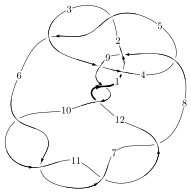
\includegraphics[width=112pt]{../../../GIT/diagram.site/Diagrams/png/1649_12a_0848.png}\\
\ \ \ A knot diagram\footnotemark}&
\allowdisplaybreaks
\textbf{Linearized knot diagam} \\
\cline{2-2}
 &
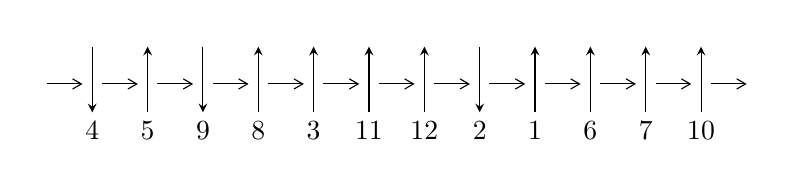
\begin{tikzpicture}[x=20pt, y=17pt]
	% nodes
	\node (C0) at (0, 0) {};
	\node (C1) at (1, 0) {};
	\node (C1U) at (1, +1) {};
	\node (C1D) at (1, -1) {4};

	\node (C2) at (2, 0) {};
	\node (C2U) at (2, +1) {};
	\node (C2D) at (2, -1) {5};

	\node (C3) at (3, 0) {};
	\node (C3U) at (3, +1) {};
	\node (C3D) at (3, -1) {9};

	\node (C4) at (4, 0) {};
	\node (C4U) at (4, +1) {};
	\node (C4D) at (4, -1) {8};

	\node (C5) at (5, 0) {};
	\node (C5U) at (5, +1) {};
	\node (C5D) at (5, -1) {3};

	\node (C6) at (6, 0) {};
	\node (C6U) at (6, +1) {};
	\node (C6D) at (6, -1) {11};

	\node (C7) at (7, 0) {};
	\node (C7U) at (7, +1) {};
	\node (C7D) at (7, -1) {12};

	\node (C8) at (8, 0) {};
	\node (C8U) at (8, +1) {};
	\node (C8D) at (8, -1) {2};

	\node (C9) at (9, 0) {};
	\node (C9U) at (9, +1) {};
	\node (C9D) at (9, -1) {1};

	\node (C10) at (10, 0) {};
	\node (C10U) at (10, +1) {};
	\node (C10D) at (10, -1) {6};

	\node (C11) at (11, 0) {};
	\node (C11U) at (11, +1) {};
	\node (C11D) at (11, -1) {7};

	\node (C12) at (12, 0) {};
	\node (C12U) at (12, +1) {};
	\node (C12D) at (12, -1) {10};
	\node (C13) at (13, 0) {};

	% arrows
	\draw[->,>={angle 60}]
	(C0) edge (C1) (C1) edge (C2) (C2) edge (C3) (C3) edge (C4) (C4) edge (C5) (C5) edge (C6) (C6) edge (C7) (C7) edge (C8) (C8) edge (C9) (C9) edge (C10) (C10) edge (C11) (C11) edge (C12) (C12) edge (C13) ;	\draw[->,>=stealth]
	(C1U) edge (C1D) (C2D) edge (C2U) (C3U) edge (C3D) (C4D) edge (C4U) (C5D) edge (C5U) (C6D) edge (C6U) (C7D) edge (C7U) (C8U) edge (C8D) (C9D) edge (C9U) (C10D) edge (C10U) (C11D) edge (C11U) (C12D) edge (C12U) ;
	\end{tikzpicture} \\
\hhline{~~} \\& 
\textbf{Solving Sequence} \\ \cline{2-2} 
 &
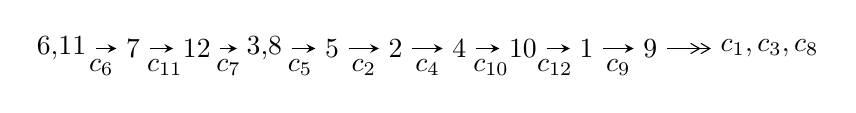
\begin{tikzpicture}[x=23pt, y=7pt]
	% node
	\node (A0) at (-1/8, 0) {6,11};
	\node (A1) at (1, 0) {7};
	\node (A2) at (2, 0) {12};
	\node (A3) at (49/16, 0) {3,8};
	\node (A4) at (33/8, 0) {5};
	\node (A5) at (41/8, 0) {2};
	\node (A6) at (49/8, 0) {4};
	\node (A7) at (57/8, 0) {10};
	\node (A8) at (65/8, 0) {1};
	\node (A9) at (73/8, 0) {9};
	\node (C1) at (1/2, -1) {$c_{6}$};
	\node (C2) at (3/2, -1) {$c_{11}$};
	\node (C3) at (5/2, -1) {$c_{7}$};
	\node (C4) at (29/8, -1) {$c_{5}$};
	\node (C5) at (37/8, -1) {$c_{2}$};
	\node (C6) at (45/8, -1) {$c_{4}$};
	\node (C7) at (53/8, -1) {$c_{10}$};
	\node (C8) at (61/8, -1) {$c_{12}$};
	\node (C9) at (69/8, -1) {$c_{9}$};
	\node (A10) at (11, 0) {$c_{1},c_{3},c_{8}$};

	% edge
	\draw[->,>=stealth]	
	(A0) edge (A1) (A1) edge (A2) (A2) edge (A3) (A3) edge (A4) (A4) edge (A5) (A5) edge (A6) (A6) edge (A7) (A7) edge (A8) (A8) edge (A9) ;
	\draw[->>,>={angle 60}]	
	(A9) edge (A10);
\end{tikzpicture} \\ 

\end{tabular} \\

\footnotetext{
The image of knot diagram is generated by the software ``\textbf{Draw programme}" developed by Andrew Bartholomew(\url{http://www.layer8.co.uk/maths/draw/index.htm\#Running-draw}), where we modified some parts for our purpose(\url{https://github.com/CATsTAILs/LinksPainter}).
}\phantom \\ \newline 
\centering \textbf{Ideals for irreducible components\footnotemark of $X_{\text{par}}$} 
 
\begin{align*}
I^u_{1}&=\langle 
6.79509\times10^{25} u^{81}-1.87697\times10^{26} u^{80}+\cdots+3.12829\times10^{26} b+3.70010\times10^{26},\\
\phantom{I^u_{1}}&\phantom{= \langle  }-1.25500\times10^{27} u^{81}+4.42966\times10^{27} u^{80}+\cdots+3.12829\times10^{26} a-3.60905\times10^{27},\;u^{82}-2 u^{81}+\cdots+5 u+1\rangle \\
I^u_{2}&=\langle 
b-1,\;a- u+4,\;u^2- u-1\rangle \\
\\
\end{align*}
\raggedright * 2 irreducible components of $\dim_{\mathbb{C}}=0$, with total 84 representations.\\
\footnotetext{All coefficients of polynomials are rational numbers. But the coefficients are sometimes approximated in decimal forms when there is not enough margin.}
\newpage
\renewcommand{\arraystretch}{1}
\centering \section*{I. $I^u_{1}= \langle 6.80\times10^{25} u^{81}-1.88\times10^{26} u^{80}+\cdots+3.13\times10^{26} b+3.70\times10^{26},\;-1.26\times10^{27} u^{81}+4.43\times10^{27} u^{80}+\cdots+3.13\times10^{26} a-3.61\times10^{27},\;u^{82}-2 u^{81}+\cdots+5 u+1 \rangle$}
\flushleft \textbf{(i) Arc colorings}\\
\begin{tabular}{m{7pt} m{180pt} m{7pt} m{180pt} }
\flushright $a_{6}=$&$\begin{pmatrix}1\\0\end{pmatrix}$ \\
\flushright $a_{11}=$&$\begin{pmatrix}0\\u\end{pmatrix}$ \\
\flushright $a_{7}=$&$\begin{pmatrix}1\\- u^2\end{pmatrix}$ \\
\flushright $a_{12}=$&$\begin{pmatrix}u\\- u^3+u\end{pmatrix}$ \\
\flushright $a_{3}=$&$\begin{pmatrix}4.01178 u^{81}-14.1600 u^{80}+\cdots+49.3240 u+11.5368\\-0.217214 u^{81}+0.599999 u^{80}+\cdots-0.525322 u-1.18279\end{pmatrix}$ \\
\flushright $a_{8}=$&$\begin{pmatrix}- u^2+1\\u^4-2 u^2\end{pmatrix}$ \\
\flushright $a_{5}=$&$\begin{pmatrix}-3.73565 u^{81}+13.7600 u^{80}+\cdots-50.1788 u-10.6699\\0.131143 u^{81}-0.600003 u^{80}+\cdots+0.898711 u+1.26886\end{pmatrix}$ \\
\flushright $a_{2}=$&$\begin{pmatrix}1.23051 u^{81}-0.600008 u^{80}+\cdots-4.81570 u+0.0834147\\-0.827859 u^{81}+7.27353\times10^{-6} u^{80}+\cdots+4.25322 u+0.827859\end{pmatrix}$ \\
\flushright $a_{4}=$&$\begin{pmatrix}-3.69924 u^{81}+10.1600 u^{80}+\cdots-30.3291 u-6.30999\\0.0984670 u^{81}+1.40003 u^{80}+\cdots-9.34157 u-1.49847\end{pmatrix}$ \\
\flushright $a_{10}=$&$\begin{pmatrix}- u\\u\end{pmatrix}$ \\
\flushright $a_{1}=$&$\begin{pmatrix}- u^5+2 u^3+u\\u^5-3 u^3+u\end{pmatrix}$ \\
\flushright $a_{9}=$&$\begin{pmatrix}- u^9+4 u^7-3 u^5-2 u^3- u\\u^9-5 u^7+7 u^5-2 u^3+u\end{pmatrix}$\\&\end{tabular}
\flushleft \textbf{(ii) Obstruction class $= -1$}\\~\\
\flushleft \textbf{(iii) Cusp Shapes $= -\frac{12431619809245966583934679162}{312829021899527050766390809} u^{81}+\frac{35624969286962567890354505997}{312829021899527050766390809} u^{80}+\cdots-\frac{83891237795955352645480927062}{312829021899527050766390809} u-\frac{25270533899815883781765835149}{312829021899527050766390809}$}\\~\\
\newpage\renewcommand{\arraystretch}{1}
\flushleft \textbf{(iv) u-Polynomials at the component}\newline \\
\begin{tabular}{m{50pt}|m{274pt}}
Crossings & \hspace{64pt}u-Polynomials at each crossing \\
\hline $$\begin{aligned}c_{1}\end{aligned}$$&$\begin{aligned}
&u^{82}-13 u^{81}+\cdots+20 u+4
\end{aligned}$\\
\hline $$\begin{aligned}c_{2},c_{5}\end{aligned}$$&$\begin{aligned}
&u^{82}+3 u^{81}+\cdots-10 u+1
\end{aligned}$\\
\hline $$\begin{aligned}c_{3}\end{aligned}$$&$\begin{aligned}
&u^{82}-41 u^{80}+\cdots-320 u+56
\end{aligned}$\\
\hline $$\begin{aligned}c_{4}\end{aligned}$$&$\begin{aligned}
&u^{82}-2 u^{81}+\cdots+9 u+1
\end{aligned}$\\
\hline $$\begin{aligned}c_{6},c_{7},c_{10}\\c_{11}\end{aligned}$$&$\begin{aligned}
&u^{82}+2 u^{81}+\cdots-5 u+1
\end{aligned}$\\
\hline $$\begin{aligned}c_{8}\end{aligned}$$&$\begin{aligned}
&u^{82}+4 u^{81}+\cdots+u+1
\end{aligned}$\\
\hline $$\begin{aligned}c_{9},c_{12}\end{aligned}$$&$\begin{aligned}
&u^{82}+14 u^{81}+\cdots+13953 u+1583
\end{aligned}$\\
\hline
\end{tabular}\\~\\
\newpage\renewcommand{\arraystretch}{1}
\flushleft \textbf{(v) Riley Polynomials at the component}\newline \\
\begin{tabular}{m{50pt}|m{274pt}}
Crossings & \hspace{64pt}Riley Polynomials at each crossing \\
\hline $$\begin{aligned}c_{1}\end{aligned}$$&$\begin{aligned}
&y^{82}-15 y^{81}+\cdots-424 y+16
\end{aligned}$\\
\hline $$\begin{aligned}c_{2},c_{5}\end{aligned}$$&$\begin{aligned}
&y^{82}-49 y^{81}+\cdots-138 y+1
\end{aligned}$\\
\hline $$\begin{aligned}c_{3}\end{aligned}$$&$\begin{aligned}
&y^{82}-82 y^{81}+\cdots-254496 y+3136
\end{aligned}$\\
\hline $$\begin{aligned}c_{4}\end{aligned}$$&$\begin{aligned}
&y^{82}-78 y^{81}+\cdots-291 y+1
\end{aligned}$\\
\hline $$\begin{aligned}c_{6},c_{7},c_{10}\\c_{11}\end{aligned}$$&$\begin{aligned}
&y^{82}-90 y^{81}+\cdots-3 y+1
\end{aligned}$\\
\hline $$\begin{aligned}c_{8}\end{aligned}$$&$\begin{aligned}
&y^{82}+10 y^{81}+\cdots-3 y+1
\end{aligned}$\\
\hline $$\begin{aligned}c_{9},c_{12}\end{aligned}$$&$\begin{aligned}
&y^{82}+54 y^{81}+\cdots+132694021 y+2505889
\end{aligned}$\\
\hline
\end{tabular}\\~\\
\newpage\flushleft \textbf{(vi) Complex Volumes and Cusp Shapes}
$$\begin{array}{c|c|c}  
\text{Solutions to }I^u_{1}& \I (\text{vol} + \sqrt{-1}CS) & \text{Cusp shape}\\
 \hline 
\begin{aligned}
u &= -0.870995\phantom{ +0.000000I} \\
a &= -1.72046\phantom{ +0.000000I} \\
b &= \phantom{-}0.696147\phantom{ +0.000000I}\end{aligned}
 & \phantom{-}1.59278\phantom{ +0.000000I} & \phantom{-0.000000 } 0 \\ \hline\begin{aligned}
u &= \phantom{-}0.811511 + 0.271221 I \\
a &= -2.19736 + 0.75030 I \\
b &= \phantom{-}1.239060 + 0.452098 I\end{aligned}
 & \phantom{-}4.42119 + 8.06572 I & \phantom{-0.000000 } 0 \\ \hline\begin{aligned}
u &= \phantom{-}0.811511 - 0.271221 I \\
a &= -2.19736 - 0.75030 I \\
b &= \phantom{-}1.239060 - 0.452098 I\end{aligned}
 & \phantom{-}4.42119 - 8.06572 I & \phantom{-0.000000 } 0 \\ \hline\begin{aligned}
u &= -0.594864 + 0.611462 I \\
a &= -1.22801 - 2.05470 I \\
b &= \phantom{-}1.31195 - 0.61880 I\end{aligned}
 & -1.30842 - 13.62090 I & \phantom{-0.000000 } 0 \\ \hline\begin{aligned}
u &= -0.594864 - 0.611462 I \\
a &= -1.22801 + 2.05470 I \\
b &= \phantom{-}1.31195 + 0.61880 I\end{aligned}
 & -1.30842 + 13.62090 I & \phantom{-0.000000 } 0 \\ \hline\begin{aligned}
u &= -0.764155 + 0.376279 I \\
a &= -1.13837 - 1.23153 I \\
b &= \phantom{-}1.113830 + 0.304908 I\end{aligned}
 & \phantom{-}3.83447 + 1.89000 I & \phantom{-0.000000 } 0 \\ \hline\begin{aligned}
u &= -0.764155 - 0.376279 I \\
a &= -1.13837 + 1.23153 I \\
b &= \phantom{-}1.113830 - 0.304908 I\end{aligned}
 & \phantom{-}3.83447 - 1.89000 I & \phantom{-0.000000 } 0 \\ \hline\begin{aligned}
u &= \phantom{-}0.610557 + 0.592676 I \\
a &= -1.25430 + 1.40948 I \\
b &= \phantom{-}0.964576 + 0.401078 I\end{aligned}
 & -2.62652 + 5.81470 I & \phantom{-0.000000 } 0 \\ \hline\begin{aligned}
u &= \phantom{-}0.610557 - 0.592676 I \\
a &= -1.25430 - 1.40948 I \\
b &= \phantom{-}0.964576 - 0.401078 I\end{aligned}
 & -2.62652 - 5.81470 I & \phantom{-0.000000 } 0 \\ \hline\begin{aligned}
u &= -0.556885 + 0.597439 I \\
a &= \phantom{-}1.214540 + 0.434604 I \\
b &= \phantom{-}0.184378 + 1.180630 I\end{aligned}
 & -4.87343 - 7.34073 I & \phantom{-0.000000 } 0\\
 \hline 
 \end{array}$$\newpage$$\begin{array}{c|c|c}  
\text{Solutions to }I^u_{1}& \I (\text{vol} + \sqrt{-1}CS) & \text{Cusp shape}\\
 \hline 
\begin{aligned}
u &= -0.556885 - 0.597439 I \\
a &= \phantom{-}1.214540 - 0.434604 I \\
b &= \phantom{-}0.184378 - 1.180630 I\end{aligned}
 & -4.87343 + 7.34073 I & \phantom{-0.000000 } 0 \\ \hline\begin{aligned}
u &= \phantom{-}0.528286 + 0.620135 I \\
a &= \phantom{-}0.124296 + 0.097755 I \\
b &= \phantom{-}0.406875 - 0.376887 I\end{aligned}
 & -4.10622 + 2.32469 I & \phantom{-0.000000 } 0 \\ \hline\begin{aligned}
u &= \phantom{-}0.528286 - 0.620135 I \\
a &= \phantom{-}0.124296 - 0.097755 I \\
b &= \phantom{-}0.406875 + 0.376887 I\end{aligned}
 & -4.10622 - 2.32469 I & \phantom{-0.000000 } 0 \\ \hline\begin{aligned}
u &= \phantom{-}0.462275 + 0.639883 I \\
a &= -0.332685 + 0.621312 I \\
b &= \phantom{-}0.536469 + 0.377022 I\end{aligned}
 & -4.30287 + 1.94000 I & \phantom{-0.000000 } 0 \\ \hline\begin{aligned}
u &= \phantom{-}0.462275 - 0.639883 I \\
a &= -0.332685 - 0.621312 I \\
b &= \phantom{-}0.536469 - 0.377022 I\end{aligned}
 & -4.30287 - 1.94000 I & \phantom{-0.000000 } 0 \\ \hline\begin{aligned}
u &= -0.543646 + 0.553436 I \\
a &= \phantom{-}0.95361 + 2.22060 I \\
b &= -1.18611 + 0.80921 I\end{aligned}
 & \phantom{-}0.40590 - 5.34297 I & \phantom{-}6.00000 + 9.52274 I \\ \hline\begin{aligned}
u &= -0.543646 - 0.553436 I \\
a &= \phantom{-}0.95361 - 2.22060 I \\
b &= -1.18611 - 0.80921 I\end{aligned}
 & \phantom{-}0.40590 + 5.34297 I & \phantom{-}6.00000 - 9.52274 I \\ \hline\begin{aligned}
u &= \phantom{-}0.513004 + 0.563882 I \\
a &= \phantom{-}0.90964 - 3.31132 I \\
b &= -0.978158 - 0.173023 I\end{aligned}
 & -1.20160 + 2.58017 I & \phantom{-}6.00000 + 7.53733 I \\ \hline\begin{aligned}
u &= \phantom{-}0.513004 - 0.563882 I \\
a &= \phantom{-}0.90964 + 3.31132 I \\
b &= -0.978158 + 0.173023 I\end{aligned}
 & -1.20160 - 2.58017 I & \phantom{-}6.00000 - 7.53733 I \\ \hline\begin{aligned}
u &= -0.384471 + 0.651387 I \\
a &= \phantom{-}0.161962 + 0.374695 I \\
b &= \phantom{-}1.28132 + 0.61475 I\end{aligned}
 & -1.93003 + 9.35126 I & \phantom{-}6.00000 - 4.19971 I\\
 \hline 
 \end{array}$$\newpage$$\begin{array}{c|c|c}  
\text{Solutions to }I^u_{1}& \I (\text{vol} + \sqrt{-1}CS) & \text{Cusp shape}\\
 \hline 
\begin{aligned}
u &= -0.384471 - 0.651387 I \\
a &= \phantom{-}0.161962 - 0.374695 I \\
b &= \phantom{-}1.28132 - 0.61475 I\end{aligned}
 & -1.93003 - 9.35126 I & \phantom{-}6.00000 + 4.19971 I \\ \hline\begin{aligned}
u &= -0.423577 + 0.616541 I \\
a &= -0.612466 - 1.070720 I \\
b &= \phantom{-}0.227379 - 1.135570 I\end{aligned}
 & -5.26621 + 3.21097 I & \phantom{-}2.08818 - 1.93788 I \\ \hline\begin{aligned}
u &= -0.423577 - 0.616541 I \\
a &= -0.612466 + 1.070720 I \\
b &= \phantom{-}0.227379 + 1.135570 I\end{aligned}
 & -5.26621 - 3.21097 I & \phantom{-}2.08818 + 1.93788 I \\ \hline\begin{aligned}
u &= \phantom{-}0.469113 + 0.564443 I \\
a &= -0.00398 + 1.58925 I \\
b &= -0.924415 + 0.181797 I\end{aligned}
 & -1.33155 + 1.29922 I & \phantom{-}5.09604 - 13.12638 I \\ \hline\begin{aligned}
u &= \phantom{-}0.469113 - 0.564443 I \\
a &= -0.00398 - 1.58925 I \\
b &= -0.924415 - 0.181797 I\end{aligned}
 & -1.33155 - 1.29922 I & \phantom{-}5.09604 + 13.12638 I \\ \hline\begin{aligned}
u &= \phantom{-}0.354693 + 0.630587 I \\
a &= -0.277083 - 0.223148 I \\
b &= \phantom{-}0.879813 - 0.422336 I\end{aligned}
 & -3.37714 - 1.66121 I & \phantom{-}1.62414 + 2.54415 I \\ \hline\begin{aligned}
u &= \phantom{-}0.354693 - 0.630587 I \\
a &= -0.277083 + 0.223148 I \\
b &= \phantom{-}0.879813 + 0.422336 I\end{aligned}
 & -3.37714 + 1.66121 I & \phantom{-}1.62414 - 2.54415 I \\ \hline\begin{aligned}
u &= -0.501466 + 0.511705 I \\
a &= \phantom{-}0.13756 + 1.63725 I \\
b &= -1.55579 - 0.07559 I\end{aligned}
 & \phantom{-}1.77607 - 1.77523 I & \phantom{-}11.62947 + 4.03448 I \\ \hline\begin{aligned}
u &= -0.501466 - 0.511705 I \\
a &= \phantom{-}0.13756 - 1.63725 I \\
b &= -1.55579 + 0.07559 I\end{aligned}
 & \phantom{-}1.77607 + 1.77523 I & \phantom{-}11.62947 - 4.03448 I \\ \hline\begin{aligned}
u &= -0.427166 + 0.550491 I \\
a &= -0.978268 - 0.385975 I \\
b &= -1.083790 - 0.789192 I\end{aligned}
 & \phantom{-}0.06386 + 1.53089 I & \phantom{-}8.01853 - 2.55528 I\\
 \hline 
 \end{array}$$\newpage$$\begin{array}{c|c|c}  
\text{Solutions to }I^u_{1}& \I (\text{vol} + \sqrt{-1}CS) & \text{Cusp shape}\\
 \hline 
\begin{aligned}
u &= -0.427166 - 0.550491 I \\
a &= -0.978268 + 0.385975 I \\
b &= -1.083790 + 0.789192 I\end{aligned}
 & \phantom{-}0.06386 - 1.53089 I & \phantom{-}8.01853 + 2.55528 I \\ \hline\begin{aligned}
u &= \phantom{-}0.638658 + 0.225748 I \\
a &= \phantom{-}0.389590 + 0.593475 I \\
b &= -0.065745 - 0.839937 I\end{aligned}
 & \phantom{-}0.57980 + 3.50184 I & \phantom{-}9.13977 - 8.90490 I \\ \hline\begin{aligned}
u &= \phantom{-}0.638658 - 0.225748 I \\
a &= \phantom{-}0.389590 - 0.593475 I \\
b &= -0.065745 + 0.839937 I\end{aligned}
 & \phantom{-}0.57980 - 3.50184 I & \phantom{-}9.13977 + 8.90490 I \\ \hline\begin{aligned}
u &= \phantom{-}0.652505 + 0.065512 I \\
a &= \phantom{-}2.65287 - 0.29373 I \\
b &= -1.316620 - 0.452019 I\end{aligned}
 & \phantom{-}4.30182 + 1.62654 I & \phantom{-}18.7241 - 4.7341 I \\ \hline\begin{aligned}
u &= \phantom{-}0.652505 - 0.065512 I \\
a &= \phantom{-}2.65287 + 0.29373 I \\
b &= -1.316620 + 0.452019 I\end{aligned}
 & \phantom{-}4.30182 - 1.62654 I & \phantom{-}18.7241 + 4.7341 I \\ \hline\begin{aligned}
u &= -0.053845 + 0.582038 I \\
a &= -0.014038 - 0.437876 I \\
b &= \phantom{-}1.139860 - 0.413488 I\end{aligned}
 & \phantom{-}1.64921 - 5.15659 I & \phantom{-}5.38071 + 6.28870 I \\ \hline\begin{aligned}
u &= -0.053845 - 0.582038 I \\
a &= -0.014038 + 0.437876 I \\
b &= \phantom{-}1.139860 + 0.413488 I\end{aligned}
 & \phantom{-}1.64921 + 5.15659 I & \phantom{-}5.38071 - 6.28870 I \\ \hline\begin{aligned}
u &= -1.42911 + 0.12607 I \\
a &= -1.021550 - 0.129914 I \\
b &= \phantom{-}0.738343 + 0.519400 I\end{aligned}
 & \phantom{-}2.22829 - 0.95699 I & \phantom{-0.000000 } 0 \\ \hline\begin{aligned}
u &= -1.42911 - 0.12607 I \\
a &= -1.021550 + 0.129914 I \\
b &= \phantom{-}0.738343 - 0.519400 I\end{aligned}
 & \phantom{-}2.22829 + 0.95699 I & \phantom{-0.000000 } 0 \\ \hline\begin{aligned}
u &= \phantom{-}1.42513 + 0.16645 I \\
a &= -0.951642 + 0.179384 I \\
b &= \phantom{-}1.230580 - 0.607759 I\end{aligned}
 & \phantom{-}3.83137 - 6.45058 I & \phantom{-0.000000 } 0\\
 \hline 
 \end{array}$$\newpage$$\begin{array}{c|c|c}  
\text{Solutions to }I^u_{1}& \I (\text{vol} + \sqrt{-1}CS) & \text{Cusp shape}\\
 \hline 
\begin{aligned}
u &= \phantom{-}1.42513 - 0.16645 I \\
a &= -0.951642 - 0.179384 I \\
b &= \phantom{-}1.230580 + 0.607759 I\end{aligned}
 & \phantom{-}3.83137 + 6.45058 I & \phantom{-0.000000 } 0 \\ \hline\begin{aligned}
u &= -0.545660 + 0.113928 I \\
a &= -0.983595 + 0.442700 I \\
b &= -0.1046930 - 0.0437336 I\end{aligned}
 & \phantom{-}0.978391 - 0.167632 I & \phantom{-}10.95193 + 1.32595 I \\ \hline\begin{aligned}
u &= -0.545660 - 0.113928 I \\
a &= -0.983595 - 0.442700 I \\
b &= -0.1046930 + 0.0437336 I\end{aligned}
 & \phantom{-}0.978391 + 0.167632 I & \phantom{-}10.95193 - 1.32595 I \\ \hline\begin{aligned}
u &= -0.529899\phantom{ +0.000000I} \\
a &= \phantom{-}10.3142\phantom{ +0.000000I} \\
b &= -1.02032\phantom{ +0.000000I}\end{aligned}
 & \phantom{-}2.51211\phantom{ +0.000000I} & -88.5500\phantom{ +0.000000I} \\ \hline\begin{aligned}
u &= \phantom{-}1.47193 + 0.16091 I \\
a &= -0.855076 + 0.061099 I \\
b &= \phantom{-}0.297685 + 1.084440 I\end{aligned}
 & \phantom{-}0.865552 - 0.485531 I & \phantom{-0.000000 } 0 \\ \hline\begin{aligned}
u &= \phantom{-}1.47193 - 0.16091 I \\
a &= -0.855076 - 0.061099 I \\
b &= \phantom{-}0.297685 - 1.084440 I\end{aligned}
 & \phantom{-}0.865552 + 0.485531 I & \phantom{-0.000000 } 0 \\ \hline\begin{aligned}
u &= -1.48145 + 0.19094 I \\
a &= -0.844562 - 0.272193 I \\
b &= \phantom{-}0.669605 - 0.422650 I\end{aligned}
 & \phantom{-}2.01541 - 4.91638 I & \phantom{-0.000000 } 0 \\ \hline\begin{aligned}
u &= -1.48145 - 0.19094 I \\
a &= -0.844562 + 0.272193 I \\
b &= \phantom{-}0.669605 + 0.422650 I\end{aligned}
 & \phantom{-}2.01541 + 4.91638 I & \phantom{-0.000000 } 0 \\ \hline\begin{aligned}
u &= \phantom{-}1.50668 + 0.13219 I \\
a &= -0.036896 - 0.447336 I \\
b &= -0.940587 + 0.842768 I\end{aligned}
 & \phantom{-}6.42569 + 0.77348 I & \phantom{-0.000000 } 0 \\ \hline\begin{aligned}
u &= \phantom{-}1.50668 - 0.13219 I \\
a &= -0.036896 + 0.447336 I \\
b &= -0.940587 - 0.842768 I\end{aligned}
 & \phantom{-}6.42569 - 0.77348 I & \phantom{-0.000000 } 0\\
 \hline 
 \end{array}$$\newpage$$\begin{array}{c|c|c}  
\text{Solutions to }I^u_{1}& \I (\text{vol} + \sqrt{-1}CS) & \text{Cusp shape}\\
 \hline 
\begin{aligned}
u &= -1.51364 + 0.15219 I \\
a &= \phantom{-}0.536167 - 1.247610 I \\
b &= -0.866187 - 0.214071 I\end{aligned}
 & \phantom{-}5.21063 - 3.80691 I & \phantom{-0.000000 } 0 \\ \hline\begin{aligned}
u &= -1.51364 - 0.15219 I \\
a &= \phantom{-}0.536167 + 1.247610 I \\
b &= -0.866187 + 0.214071 I\end{aligned}
 & \phantom{-}5.21063 + 3.80691 I & \phantom{-0.000000 } 0 \\ \hline\begin{aligned}
u &= -1.53024 + 0.16174 I \\
a &= \phantom{-}2.19828 + 2.75110 I \\
b &= -1.021300 + 0.173147 I\end{aligned}
 & \phantom{-}5.57532 - 5.16892 I & \phantom{-0.000000 } 0 \\ \hline\begin{aligned}
u &= -1.53024 - 0.16174 I \\
a &= \phantom{-}2.19828 - 2.75110 I \\
b &= -1.021300 - 0.173147 I\end{aligned}
 & \phantom{-}5.57532 + 5.16892 I & \phantom{-0.000000 } 0 \\ \hline\begin{aligned}
u &= -1.52923 + 0.18520 I \\
a &= -0.206185 - 0.261817 I \\
b &= \phantom{-}0.296189 + 0.412108 I\end{aligned}
 & \phantom{-}2.67887 - 5.22504 I & \phantom{-0.000000 } 0 \\ \hline\begin{aligned}
u &= -1.52923 - 0.18520 I \\
a &= -0.206185 + 0.261817 I \\
b &= \phantom{-}0.296189 - 0.412108 I\end{aligned}
 & \phantom{-}2.67887 + 5.22504 I & \phantom{-0.000000 } 0 \\ \hline\begin{aligned}
u &= \phantom{-}1.54149 + 0.02620 I \\
a &= -0.413194 - 0.502741 I \\
b &= -0.273232 - 0.149623 I\end{aligned}
 & \phantom{-}8.01688 + 0.66095 I & \phantom{-0.000000 } 0 \\ \hline\begin{aligned}
u &= \phantom{-}1.54149 - 0.02620 I \\
a &= -0.413194 + 0.502741 I \\
b &= -0.273232 + 0.149623 I\end{aligned}
 & \phantom{-}8.01688 - 0.66095 I & \phantom{-0.000000 } 0 \\ \hline\begin{aligned}
u &= \phantom{-}1.53502 + 0.14471 I \\
a &= \phantom{-}1.76397 - 1.36906 I \\
b &= -1.62122 + 0.15951 I\end{aligned}
 & \phantom{-}8.58492 + 4.10520 I & \phantom{-0.000000 } 0 \\ \hline\begin{aligned}
u &= \phantom{-}1.53502 - 0.14471 I \\
a &= \phantom{-}1.76397 + 1.36906 I \\
b &= -1.62122 - 0.15951 I\end{aligned}
 & \phantom{-}8.58492 - 4.10520 I & \phantom{-0.000000 } 0\\
 \hline 
 \end{array}$$\newpage$$\begin{array}{c|c|c}  
\text{Solutions to }I^u_{1}& \I (\text{vol} + \sqrt{-1}CS) & \text{Cusp shape}\\
 \hline 
\begin{aligned}
u &= \phantom{-}1.54999\phantom{ +0.000000I} \\
a &= \phantom{-}5.72235\phantom{ +0.000000I} \\
b &= -1.07156\phantom{ +0.000000I}\end{aligned}
 & \phantom{-}9.62835\phantom{ +0.000000I} & \phantom{-0.000000 } 0 \\ \hline\begin{aligned}
u &= \phantom{-}1.54264 + 0.16225 I \\
a &= \phantom{-}1.98586 - 1.16029 I \\
b &= -1.25596 - 0.83173 I\end{aligned}
 & \phantom{-}7.35240 + 7.92215 I & \phantom{-0.000000 } 0 \\ \hline\begin{aligned}
u &= \phantom{-}1.54264 - 0.16225 I \\
a &= \phantom{-}1.98586 + 1.16029 I \\
b &= -1.25596 + 0.83173 I\end{aligned}
 & \phantom{-}7.35240 - 7.92215 I & \phantom{-0.000000 } 0 \\ \hline\begin{aligned}
u &= \phantom{-}1.54406 + 0.18057 I \\
a &= \phantom{-}0.898342 + 0.570588 I \\
b &= \phantom{-}0.148551 - 1.220200 I\end{aligned}
 & \phantom{-}2.09607 + 10.16370 I & \phantom{-0.000000 } 0 \\ \hline\begin{aligned}
u &= \phantom{-}1.54406 - 0.18057 I \\
a &= \phantom{-}0.898342 - 0.570588 I \\
b &= \phantom{-}0.148551 + 1.220200 I\end{aligned}
 & \phantom{-}2.09607 - 10.16370 I & \phantom{-0.000000 } 0 \\ \hline\begin{aligned}
u &= -1.56208 + 0.04407 I \\
a &= \phantom{-}0.356577 - 1.009890 I \\
b &= -0.205192 + 0.989853 I\end{aligned}
 & \phantom{-}8.00277 - 4.37968 I & \phantom{-0.000000 } 0 \\ \hline\begin{aligned}
u &= -1.56208 - 0.04407 I \\
a &= \phantom{-}0.356577 + 1.009890 I \\
b &= -0.205192 - 0.989853 I\end{aligned}
 & \phantom{-}8.00277 + 4.37968 I & \phantom{-0.000000 } 0 \\ \hline\begin{aligned}
u &= -1.56847 + 0.01217 I \\
a &= \phantom{-}2.90549 - 0.18562 I \\
b &= -1.44541 + 0.51761 I\end{aligned}
 & \phantom{-}11.82620 - 1.87309 I & \phantom{-0.000000 } 0 \\ \hline\begin{aligned}
u &= -1.56847 - 0.01217 I \\
a &= \phantom{-}2.90549 + 0.18562 I \\
b &= -1.44541 - 0.51761 I\end{aligned}
 & \phantom{-}11.82620 + 1.87309 I & \phantom{-0.000000 } 0 \\ \hline\begin{aligned}
u &= \phantom{-}1.55988 + 0.18904 I \\
a &= -2.19841 + 1.29679 I \\
b &= \phantom{-}1.33759 + 0.61959 I\end{aligned}
 & \phantom{-}5.8572 + 16.5563 I & \phantom{-0.000000 } 0\\
 \hline 
 \end{array}$$\newpage$$\begin{array}{c|c|c}  
\text{Solutions to }I^u_{1}& \I (\text{vol} + \sqrt{-1}CS) & \text{Cusp shape}\\
 \hline 
\begin{aligned}
u &= \phantom{-}1.55988 - 0.18904 I \\
a &= -2.19841 - 1.29679 I \\
b &= \phantom{-}1.33759 - 0.61959 I\end{aligned}
 & \phantom{-}5.8572 - 16.5563 I & \phantom{-0.000000 } 0 \\ \hline\begin{aligned}
u &= -1.56748 + 0.18297 I \\
a &= -1.93274 - 0.91566 I \\
b &= \phantom{-}1.026650 - 0.384762 I\end{aligned}
 & \phantom{-}4.64101 - 8.66957 I & \phantom{-0.000000 } 0 \\ \hline\begin{aligned}
u &= -1.56748 - 0.18297 I \\
a &= -1.93274 + 0.91566 I \\
b &= \phantom{-}1.026650 + 0.384762 I\end{aligned}
 & \phantom{-}4.64101 + 8.66957 I & \phantom{-0.000000 } 0 \\ \hline\begin{aligned}
u &= \phantom{-}0.064511 + 0.412780 I \\
a &= -0.902893 + 0.694446 I \\
b &= \phantom{-}0.152912 + 0.585524 I\end{aligned}
 & -1.19387 - 1.28666 I & -0.50594 + 1.92491 I \\ \hline\begin{aligned}
u &= \phantom{-}0.064511 - 0.412780 I \\
a &= -0.902893 - 0.694446 I \\
b &= \phantom{-}0.152912 - 0.585524 I\end{aligned}
 & -1.19387 + 1.28666 I & -0.50594 - 1.92491 I \\ \hline\begin{aligned}
u &= -1.60578 + 0.05889 I \\
a &= -2.75309 - 0.20122 I \\
b &= \phantom{-}1.313760 - 0.435079 I\end{aligned}
 & \phantom{-}12.6240 - 9.1945 I & \phantom{-0.000000 } 0 \\ \hline\begin{aligned}
u &= -1.60578 - 0.05889 I \\
a &= -2.75309 + 0.20122 I \\
b &= \phantom{-}1.313760 + 0.435079 I\end{aligned}
 & \phantom{-}12.6240 + 9.1945 I & \phantom{-0.000000 } 0 \\ \hline\begin{aligned}
u &= \phantom{-}1.60958 + 0.08865 I \\
a &= -2.02010 + 0.86926 I \\
b &= \phantom{-}1.157150 - 0.210437 I\end{aligned}
 & \phantom{-}11.93040 - 0.22921 I & \phantom{-0.000000 } 0 \\ \hline\begin{aligned}
u &= \phantom{-}1.60958 - 0.08865 I \\
a &= -2.02010 - 0.86926 I \\
b &= \phantom{-}1.157150 + 0.210437 I\end{aligned}
 & \phantom{-}11.93040 + 0.22921 I & \phantom{-0.000000 } 0 \\ \hline\begin{aligned}
u &= \phantom{-}1.64214\phantom{ +0.000000I} \\
a &= -2.06417\phantom{ +0.000000I} \\
b &= \phantom{-}0.911522\phantom{ +0.000000I}\end{aligned}
 & \phantom{-}10.2733\phantom{ +0.000000I} & \phantom{-0.000000 } 0\\
 \hline 
 \end{array}$$\newpage$$\begin{array}{c|c|c}  
\text{Solutions to }I^u_{1}& \I (\text{vol} + \sqrt{-1}CS) & \text{Cusp shape}\\
 \hline 
\begin{aligned}
u &= -0.153931 + 0.229405 I \\
a &= -2.65823 + 0.79988 I \\
b &= -1.068010 + 0.189730 I\end{aligned}
 & \phantom{-}1.95141 - 0.72099 I & \phantom{-}4.92941 - 0.08019 I \\ \hline\begin{aligned}
u &= -0.153931 - 0.229405 I \\
a &= -2.65823 - 0.79988 I \\
b &= -1.068010 - 0.189730 I\end{aligned}
 & \phantom{-}1.95141 + 0.72099 I & \phantom{-}4.92941 + 0.08019 I\\
 \hline 
 \end{array}$$\newpage\newpage\renewcommand{\arraystretch}{1}
\centering \section*{II. $I^u_{2}= \langle b-1,\;a- u+4,\;u^2- u-1 \rangle$}
\flushleft \textbf{(i) Arc colorings}\\
\begin{tabular}{m{7pt} m{180pt} m{7pt} m{180pt} }
\flushright $a_{6}=$&$\begin{pmatrix}1\\0\end{pmatrix}$ \\
\flushright $a_{11}=$&$\begin{pmatrix}0\\u\end{pmatrix}$ \\
\flushright $a_{7}=$&$\begin{pmatrix}1\\- u-1\end{pmatrix}$ \\
\flushright $a_{12}=$&$\begin{pmatrix}u\\- u-1\end{pmatrix}$ \\
\flushright $a_{3}=$&$\begin{pmatrix}u-4\\1\end{pmatrix}$ \\
\flushright $a_{8}=$&$\begin{pmatrix}- u\\u\end{pmatrix}$ \\
\flushright $a_{5}=$&$\begin{pmatrix}u-3\\1\end{pmatrix}$ \\
\flushright $a_{2}=$&$\begin{pmatrix}-1\\0\end{pmatrix}$ \\
\flushright $a_{4}=$&$\begin{pmatrix}u-2\\0\end{pmatrix}$ \\
\flushright $a_{10}=$&$\begin{pmatrix}- u\\u\end{pmatrix}$ \\
\flushright $a_{1}=$&$\begin{pmatrix}-1\\0\end{pmatrix}$ \\
\flushright $a_{9}=$&$\begin{pmatrix}-2 u\\u\end{pmatrix}$\\&\end{tabular}
\flushleft \textbf{(ii) Obstruction class $= 1$}\\~\\
\flushleft \textbf{(iii) Cusp Shapes $= 21$}\\~\\
\newpage\renewcommand{\arraystretch}{1}
\flushleft \textbf{(iv) u-Polynomials at the component}\newline \\
\begin{tabular}{m{50pt}|m{274pt}}
Crossings & \hspace{64pt}u-Polynomials at each crossing \\
\hline $$\begin{aligned}c_{1}\end{aligned}$$&$\begin{aligned}
&u^2
\end{aligned}$\\
\hline $$\begin{aligned}c_{2}\end{aligned}$$&$\begin{aligned}
&(u+1)^2
\end{aligned}$\\
\hline $$\begin{aligned}c_{3},c_{4},c_{6}\\c_{7},c_{8},c_{9}\end{aligned}$$&$\begin{aligned}
&u^2- u-1
\end{aligned}$\\
\hline $$\begin{aligned}c_{5}\end{aligned}$$&$\begin{aligned}
&(u-1)^2
\end{aligned}$\\
\hline $$\begin{aligned}c_{10},c_{11},c_{12}\end{aligned}$$&$\begin{aligned}
&u^2+u-1
\end{aligned}$\\
\hline
\end{tabular}\\~\\
\newpage\renewcommand{\arraystretch}{1}
\flushleft \textbf{(v) Riley Polynomials at the component}\newline \\
\begin{tabular}{m{50pt}|m{274pt}}
Crossings & \hspace{64pt}Riley Polynomials at each crossing \\
\hline $$\begin{aligned}c_{1}\end{aligned}$$&$\begin{aligned}
&y^2
\end{aligned}$\\
\hline $$\begin{aligned}c_{2},c_{5}\end{aligned}$$&$\begin{aligned}
&(y-1)^2
\end{aligned}$\\
\hline $$\begin{aligned}c_{3},c_{4},c_{6}\\c_{7},c_{8},c_{9}\\c_{10},c_{11},c_{12}\end{aligned}$$&$\begin{aligned}
&y^2-3 y+1
\end{aligned}$\\
\hline
\end{tabular}\\~\\
\newpage\flushleft \textbf{(vi) Complex Volumes and Cusp Shapes}
$$\begin{array}{c|c|c}  
\text{Solutions to }I^u_{2}& \I (\text{vol} + \sqrt{-1}CS) & \text{Cusp shape}\\
 \hline 
\begin{aligned}
u &= -0.618034\phantom{ +0.000000I} \\
a &= -4.61803\phantom{ +0.000000I} \\
b &= \phantom{-}1.00000\phantom{ +0.000000I}\end{aligned}
 & \phantom{-}2.63189\phantom{ +0.000000I} & \phantom{-}21.0000\phantom{ +0.000000I} \\ \hline\begin{aligned}
u &= \phantom{-}1.61803\phantom{ +0.000000I} \\
a &= -2.38197\phantom{ +0.000000I} \\
b &= \phantom{-}1.00000\phantom{ +0.000000I}\end{aligned}
 & \phantom{-}10.5276\phantom{ +0.000000I} & \phantom{-}21.0000\phantom{ +0.000000I}\\
 \hline 
 \end{array}$$\newpage
\newpage\renewcommand{\arraystretch}{1}
\centering \section*{ III. u-Polynomials}
\begin{tabular}{m{50pt}|m{274pt}}
Crossings & \hspace{64pt}u-Polynomials at each crossing \\
\hline $$\begin{aligned}c_{1}\end{aligned}$$&$\begin{aligned}
&u^2(u^{82}-13 u^{81}+\cdots+20 u+4)
\end{aligned}$\\
\hline $$\begin{aligned}c_{2}\end{aligned}$$&$\begin{aligned}
&((u+1)^2)(u^{82}+3 u^{81}+\cdots-10 u+1)
\end{aligned}$\\
\hline $$\begin{aligned}c_{3}\end{aligned}$$&$\begin{aligned}
&(u^2- u-1)(u^{82}-41 u^{80}+\cdots-320 u+56)
\end{aligned}$\\
\hline $$\begin{aligned}c_{4}\end{aligned}$$&$\begin{aligned}
&(u^2- u-1)(u^{82}-2 u^{81}+\cdots+9 u+1)
\end{aligned}$\\
\hline $$\begin{aligned}c_{5}\end{aligned}$$&$\begin{aligned}
&((u-1)^2)(u^{82}+3 u^{81}+\cdots-10 u+1)
\end{aligned}$\\
\hline $$\begin{aligned}c_{6},c_{7}\end{aligned}$$&$\begin{aligned}
&(u^2- u-1)(u^{82}+2 u^{81}+\cdots-5 u+1)
\end{aligned}$\\
\hline $$\begin{aligned}c_{8}\end{aligned}$$&$\begin{aligned}
&(u^2- u-1)(u^{82}+4 u^{81}+\cdots+u+1)
\end{aligned}$\\
\hline $$\begin{aligned}c_{9}\end{aligned}$$&$\begin{aligned}
&(u^2- u-1)(u^{82}+14 u^{81}+\cdots+13953 u+1583)
\end{aligned}$\\
\hline $$\begin{aligned}c_{10},c_{11}\end{aligned}$$&$\begin{aligned}
&(u^2+u-1)(u^{82}+2 u^{81}+\cdots-5 u+1)
\end{aligned}$\\
\hline $$\begin{aligned}c_{12}\end{aligned}$$&$\begin{aligned}
&(u^2+u-1)(u^{82}+14 u^{81}+\cdots+13953 u+1583)
\end{aligned}$\\
\hline
\end{tabular}\newpage\renewcommand{\arraystretch}{1}
\centering \section*{ IV. Riley Polynomials}
\begin{tabular}{m{50pt}|m{274pt}}
Crossings & \hspace{64pt}Riley Polynomials at each crossing \\
\hline $$\begin{aligned}c_{1}\end{aligned}$$&$\begin{aligned}
&y^2(y^{82}-15 y^{81}+\cdots-424 y+16)
\end{aligned}$\\
\hline $$\begin{aligned}c_{2},c_{5}\end{aligned}$$&$\begin{aligned}
&((y-1)^2)(y^{82}-49 y^{81}+\cdots-138 y+1)
\end{aligned}$\\
\hline $$\begin{aligned}c_{3}\end{aligned}$$&$\begin{aligned}
&(y^2-3 y+1)(y^{82}-82 y^{81}+\cdots-254496 y+3136)
\end{aligned}$\\
\hline $$\begin{aligned}c_{4}\end{aligned}$$&$\begin{aligned}
&(y^2-3 y+1)(y^{82}-78 y^{81}+\cdots-291 y+1)
\end{aligned}$\\
\hline $$\begin{aligned}c_{6},c_{7},c_{10}\\c_{11}\end{aligned}$$&$\begin{aligned}
&(y^2-3 y+1)(y^{82}-90 y^{81}+\cdots-3 y+1)
\end{aligned}$\\
\hline $$\begin{aligned}c_{8}\end{aligned}$$&$\begin{aligned}
&(y^2-3 y+1)(y^{82}+10 y^{81}+\cdots-3 y+1)
\end{aligned}$\\
\hline $$\begin{aligned}c_{9},c_{12}\end{aligned}$$&$\begin{aligned}
&(y^2-3 y+1)(y^{82}+54 y^{81}+\cdots+1.32694\times10^{8} y+2505889)
\end{aligned}$\\
\hline
\end{tabular}
\vskip 2pc
\end{document}